%\RequirePackage[l2tabu, orthodox]{nag}
\RequirePackage{currfile}
\documentclass[12pt]{beamer}
\graphicspath{{Imagenes/}{../Imagenes/}}
\usepackage[utf8]{inputenc}
\usepackage[spanish]{babel}
\usepackage{standalone}
\usepackage{color}
\usepackage[binary-units=true]{siunitx}
\usepackage{hyperref}
\hypersetup{
  colorlinks=true,
  linkcolor=blue,          % color of internal links (change box color with linkbordercolor)
  citecolor=green,        % color of links to bibliography
  filecolor=magenta,      % color of file links
  urlcolor=cyan,           % color of external links
  linkbordercolor={0 0 1}
}
\usepackage{xcolor, soul}
\usepackage{etoolbox}
\usepackage{amsmath}
\usepackage{amsthm}
\usepackage{physics}
\usepackage{multicol}
\usepackage{graphicx}
\usepackage{bookmark}
\usepackage{longtable}
\usepackage{graphicx}
\usepackage{tikz}
\usepackage[siunitx, RPvoltages]{circuitikz}
\usetikzlibrary{mindmap}
\usetikzlibrary{arrows, patterns, shapes, decorations.markings, decorations.pathmorphing}
\usetikzlibrary{matrix,positioning}
\tikzstyle{every picture}+=[remember picture,baseline]
\usepackage[autostyle,spanish=mexican]{csquotes}
\usepackage{pifont}
\usepackage[font=footnotesize,textfont=it]{caption}
\usepackage{tabulary}
\usepackage{booktabs}
\usepackage[outdir=./]{epstopdf}
%\usepackage{epstopdf}
\usepackage{media9}
\usepackage{multimedia}
\usepackage{bigints}
%\usepackage{enumitem}
\usepackage[os=win]{menukeys}
\usepackage{pifont}
\usepackage{pbox}
\usepackage{alltt}
\usepackage{verbatim}
\usepackage{colortbl}
\usepackage{tcolorbox}
\usepackage{fancyvrb}
\usepackage[sfdefault]{roboto}  %% Option 'sfdefault' only if the base font of the document is to be sans serif
%\usepackage[T1]{fontenc}
\setcounter{secnumdepth}{3}
\setcounter{tocdepth}{3}
\DeclareGraphicsExtensions{.pdf,.png,.jpg}
\renewcommand {\arraystretch}{1.5}
\definecolor{ao}{rgb}{0.0, 0.5, 0.0}
\definecolor{aquamarine}{rgb}{0.5, 1.0, 0.83}
\definecolor{kellygreen}{rgb}{0.3, 0.73, 0.09}
\definecolor{bisque}{rgb}{1.0, 0.89, 0.77}
\definecolor{amber}{rgb}{1.0, 0.75, 0.0}
\definecolor{armygreen}{rgb}{0.29, 0.33, 0.13}
\definecolor{alizarin}{rgb}{0.82, 0.1, 0.26}
\definecolor{cadetblue}{rgb}{0.37, 0.62, 0.63}
\newcommand*{\TitleParbox}[1]{\parbox[c]{6cm}{\raggedright #1}}%
\newcommand{\python}{\texttt{python}}
\newcommand{\textoazul}[1]{\textcolor{blue}{#1}}
\newcommand{\azulfuerte}[1]{\textcolor{blue}{\textbf{#1}}}
\newcommand{\funcionazul}[1]{\textcolor{blue}{\textbf{\texttt{#1}}}}
%\normalfont
\usepackage{ccfonts}% http://ctan.org/pkg/{ccfonts}
\usepackage[T1]{fontenc}% http://ctan.or/pkg/fontenc
\renewcommand{\rmdefault}{cmr}% cmr = Computer Modern Roman
\usefonttheme[onlymath]{serif}
\linespread{1.3}
\newcounter{saveenumi}
\newcommand{\seti}{\setcounter{saveenumi}{\value{enumi}}}
\newcommand{\conti}{\setcounter{enumi}{\value{saveenumi}}}
\newcommand{\tikzmark}[1]{\tikz[remember picture] \node[coordinate] (#1) {#1};}

\usepackage{scalerel}[2016-12-29]
\def\stretchint#1{\vcenter{\hbox{\stretchto[440]{\displaystyle\int}{#1}}}}
\def\scaleint#1{\vcenter{\hbox{\scaleto[3ex]{\displaystyle\int}{#1}}}}
\def\bs{\mkern-12mu}

\newtheorem{teo}{}[section]
\usepackage{blkarray}

%reduce el tamaño de letra de la etiqueta equations
\makeatletter
\def\maketag@@@#1{\hbox{\m@th\normalfont\small#1}}
\makeatother

%se usa para la x en itemize
\newcommand{\xmark}{\text{\ding{55}}}

%\AtBeginDocument{\setlength{\tymin}{1em}}


\definecolor{myblue}{rgb}{.8, .8, 1}

\usepackage{empheq}

\newlength\mytemplen
\newsavebox\mytempbox

\makeatletter
\newcommand\mybluebox{%
    \@ifnextchar[%]
       {\@mybluebox}%
       {\@mybluebox[0pt]}}

\def\@mybluebox[#1]{%
    \@ifnextchar[%]
       {\@@mybluebox[#1]}%
       {\@@mybluebox[#1][0pt]}}

\def\@@mybluebox[#1][#2]#3{
    \sbox\mytempbox{#3}%
    \mytemplen\ht\mytempbox
    \advance\mytemplen #1\relax
    \ht\mytempbox\mytemplen
    \mytemplen\dp\mytempbox
    \advance\mytemplen #2\relax
    \dp\mytempbox\mytemplen
    \colorbox{myblue}{\hspace{1em}\usebox{\mytempbox}\hspace{1em}}}

\makeatother



%Se usa la plantilla Warsaw modificada con spruce
\mode<presentation>
{
  \usetheme{Berlin}
  \setbeamertemplate{headline}{}
  \useoutertheme{default}
  \usecolortheme{beaver}
  \setbeamercovered{invisible}
}
%\AtBeginSection[]
%{
%\begin{frame}<beamer>{Contenido}
%\normalfont\mdseries
%\tableofcontents[currentsection]
%\end{frame}
%}

\setbeamertemplate{section in toc}[sections numbered]
\setbeamertemplate{subsection in toc}[subsections numbered]
\setbeamertemplate{subsection in toc}{\leavevmode\leftskip=3.2em\rlap{\hskip-2em\inserttocsectionnumber.\inserttocsubsectionnumber}\inserttocsubsection\par}
\setbeamercolor{section in toc}{fg=blue}
\setbeamercolor{subsection in toc}{fg=blue}
\setbeamertemplate{navigation symbols}{}
\setbeamercolor{frametitle}{fg=amber,bg=armygreen}
%\setbeamercolor{frametitle}{fg=blue,bg=ao!90!white}
\setbeamercolor{section in head/foot}{bg=gray!30,fg=red}
%\setbeamercolor{section in head}{bg=green,fg=red}
\setbeamercolor{subsection in head/foot}{bg=gray!30,fg=black}
\setbeamercolor{author in head/foot}{bg=gray!30}
\setbeamercolor{date in head/foot}{fg=blue}

%\mode<presentation>
%{
%  \usetheme{Warsaw}
%  \setbeamertemplate{headline}{}
%  %\useoutertheme{infolines}
%  \useoutertheme{default}
%  \setbeamercovered{invisible}
%  % or whatever (possibly just delete it)
%}

%\usepackage[backend=biber]{biblatex}
%\bibliography{LibrosFC.bib}
\usepackage{courier}
\usepackage{listingsutf8}
\usepackage{listings}
\usepackage{xcolor}
\usepackage{textcomp}
\usepackage{color}
\definecolor{deepblue}{rgb}{0,0,0.5}
\definecolor{brown}{rgb}{0.59, 0.29, 0.0}
\definecolor{OliveGreen}{rgb}{0,0.25,0}
% \usepackage{minted}

\DeclareCaptionFont{white}{\color{white}}
\DeclareCaptionFormat{listing}{\colorbox{gray}{\parbox{0.98\textwidth}{#1#2#3}}}
\captionsetup[lstlisting]{format=listing,labelfont=white,textfont=white}
\renewcommand{\lstlistingname}{Código}


\definecolor{Code}{rgb}{0,0,0}
\definecolor{Keywords}{rgb}{255,0,0}
\definecolor{Strings}{rgb}{255,0,255}
\definecolor{Comments}{rgb}{0,0,255}
\definecolor{Numbers}{rgb}{255,128,0}

\makeatletter

\newif\iffirstchar\firstchartrue
\newif\ifstartedbyadigit
\newif\ifprecededbyequalsign

\newcommand\processletter
{%
  \ifnum\lst@mode=\lst@Pmode%
    \iffirstchar%
        \global\startedbyadigitfalse%
      \fi
      \global\firstcharfalse%
    \fi
}

\newcommand\processdigit
{%
  \ifnum\lst@mode=\lst@Pmode%
      \iffirstchar%
        \global\startedbyadigittrue%
      \fi
      \global\firstcharfalse%
  \fi
}

\lst@AddToHook{OutputOther}%
{%
  \lst@IfLastOtherOneOf{=}
    {\global\precededbyequalsigntrue}
    {}%
}

\lst@AddToHook{Output}%
{%
  \ifprecededbyequalsign%
      \ifstartedbyadigit%
        \def\lst@thestyle{\color{orange}}%
      \fi
    \fi
  \global\firstchartrue%
  \global\startedbyadigitfalse%
  \global\precededbyequalsignfalse%
}

\lstset{ 
language=Python,                % choose the language of the code
basicstyle=\footnotesize\ttfamily,       % the size of the fonts that are used for the code
numbers=left,                   % where to put the line-numbers
numberstyle=\scriptsize,      % the size of the fonts that are used for the line-numbers
stepnumber=1,                   % the step between two line-numbers. If it is 1 each line will be numbered
numbersep=5pt,                  % how far the line-numbers are from the code
backgroundcolor=\color{white},  % choose the background color. You must add \usepackage{color}
showspaces=false,               % show spaces adding particular underscores
showstringspaces=false,         % underline spaces within strings
showtabs=false,                 % show tabs within strings adding particular underscores
frame=single,   		% adds a frame around the code
tabsize=2,  		% sets default tabsize to 2 spaces
captionpos=t,   		% sets the caption-position to bottom
breaklines=true,    	% sets automatic line breaking
breakatwhitespace=false,    % sets if automatic breaks should only happen at whitespace
escapeinside={\#},  % if you want to add a comment within your code
stringstyle =\color{OliveGreen},
%otherkeywords={{as}},             % Add keywords here
keywordstyle = \color{blue},
commentstyle = \color{black},
identifierstyle = \color{black},
literate=%
         {á}{{\'a}}1
         {é}{{\'e}}1
         {í}{{\'i}}1
         {ó}{{\'o}}1
         {ú}{{\'u}}1
%
%keywordstyle=\ttb\color{deepblue}
%fancyvrb = true,
}

\lstdefinestyle{FormattedNumber}{%
    literate={0}{{\textcolor{red}{0}}}{1}%
             {1}{{\textcolor{red}{1}}}{1}%
             {2}{{\textcolor{red}{2}}}{1}%
             {3}{{\textcolor{red}{3}}}{1}%
             {4}{{\textcolor{red}{4}}}{1}%
             {5}{{\textcolor{red}{5}}}{1}%
             {6}{{\textcolor{red}{6}}}{1}%
             {7}{{\textcolor{red}{7}}}{1}%
             {8}{{\textcolor{red}{8}}}{1}%
             {9}{{\textcolor{red}{9}}}{1}%
             {.0}{{\textcolor{red}{.0}}}{2}% Following is to ensure that only periods
             {.1}{{\textcolor{red}{.1}}}{2}% followed by a digit are changed.
             {.2}{{\textcolor{red}{.2}}}{2}%
             {.3}{{\textcolor{red}{.3}}}{2}%
             {.4}{{\textcolor{red}{.4}}}{2}%
             {.5}{{\textcolor{red}{.5}}}{2}%
             {.6}{{\textcolor{red}{.6}}}{2}%
             {.7}{{\textcolor{red}{.7}}}{2}%
             {.8}{{\textcolor{red}{.8}}}{2}%
             {.9}{{\textcolor{red}{.9}}}{2}%
             {\ }{{ }}{1}% handle the space
         ,%
          %mathescape=true
          escapeinside={__}
          }



\setbeamercolor{section in foot}{fg=white, bg=BlueViolet}
\makeatletter
\setbeamertemplate{footline}
{
  \leavevmode%
  \hbox{%
  \begin{beamercolorbox}[wd=.333333\paperwidth,ht=2.25ex,dp=1ex,center]{author in head/foot}%
    \usebeamerfont{section in /foot} {\insertsection}
  \end{beamercolorbox}%
  \begin{beamercolorbox}[wd=.333333\paperwidth,ht=2.25ex,dp=1ex,center]{title in head/foot}%
    \usebeamerfont{section in head/foot} {\insertsubsection}
  \end{beamercolorbox}%
  \begin{beamercolorbox}[wd=.333333\paperwidth,ht=2.25ex,dp=1ex,right]{date in head/foot}%
    \usebeamerfont{date in head/foot}\insertshortdate{}\hspace*{2em}
    \insertframenumber{} / \inserttotalframenumber\hspace*{2ex} 
  \end{beamercolorbox}}%
  \vskip0pt%
}
\makeatother

\title{Tema 0 - Graficación con \python}
\subtitle{Semestre 2018-1}
\author[]{M. en C. Gustavo Contreras Mayén \\ M. en C. Abraham Lima Buendía}
\institute{Facultad de Ciencias - UNAM}
\titlegraphic{
\includegraphics[width=2cm]{escudo-facultad-ciencias}\hspace*{4.75cm}~%
   
\includegraphics[width=2cm]{escudo-unam}
}
\date{\today}
\begin{document}
\maketitle
\section*{Contenido}
\frame[allowframebreaks]{\tableofcontents[currentsection, hideallsubsections]}
\fontsize{14}{14}\selectfont
\spanishdecimal{.}
\section{Graficación con \python}
\frame{\tableofcontents[currentsection, hideothersubsections]}
\subsection{Librería para graficación}
\begin{frame}
\frametitle{Graficación con \python}
Una buena parte del trabajo que tendremos que hacer como físicos es utilizar un conjunto de datos que por si solos, no van a darnos información sobre un modelo o un fenómeno, por ello, será necesario usar gráficas.
\end{frame}
\begin{frame}
\python\ incluye un módulo de graficación bastante versátil para generar gráficas y exportarlas a diferentes tipos de archivos.
\\
\medskip
La librería se llama \funcionazul{matplotlib}. Haremos algunos ejercicios para demostrar su potencia.
\end{frame}
\begin{frame}
\funcionazul{matplotlib.pyplot} es una colección de funciones de estilo de mando, de tal manera que \funcionazul{matplotlib} funciona a la manera de MATLAB.
\\
\bigskip
Cada instrucción \funcionazul{pyplot} aplica un cambio a una figura: por ejemplo, crear una figura, crear un área de trazado en una figura, trazar algunas líneas en un área de trazado, decorar con etiquetas, etc.
\end{frame}
\subsection{Gráficas básicas}
\begin{frame}[fragile]
\frametitle{Ejercicio 1}
\begin{lstlisting}[caption=Gráfica básica, basicstyle=\linespread{1.2}\ttfamily\small, columns=fullflexible]
import matplotlib.pyplot as plt

plt.plot([1, 2, 3, 4])
plt.ylabel('algunos numeros')
plt.show()
\end{lstlisting}
\end{frame}
\begin{frame}[fragile]
\frametitle{Ejercicio 1}
\begin{figure}
	\centering
	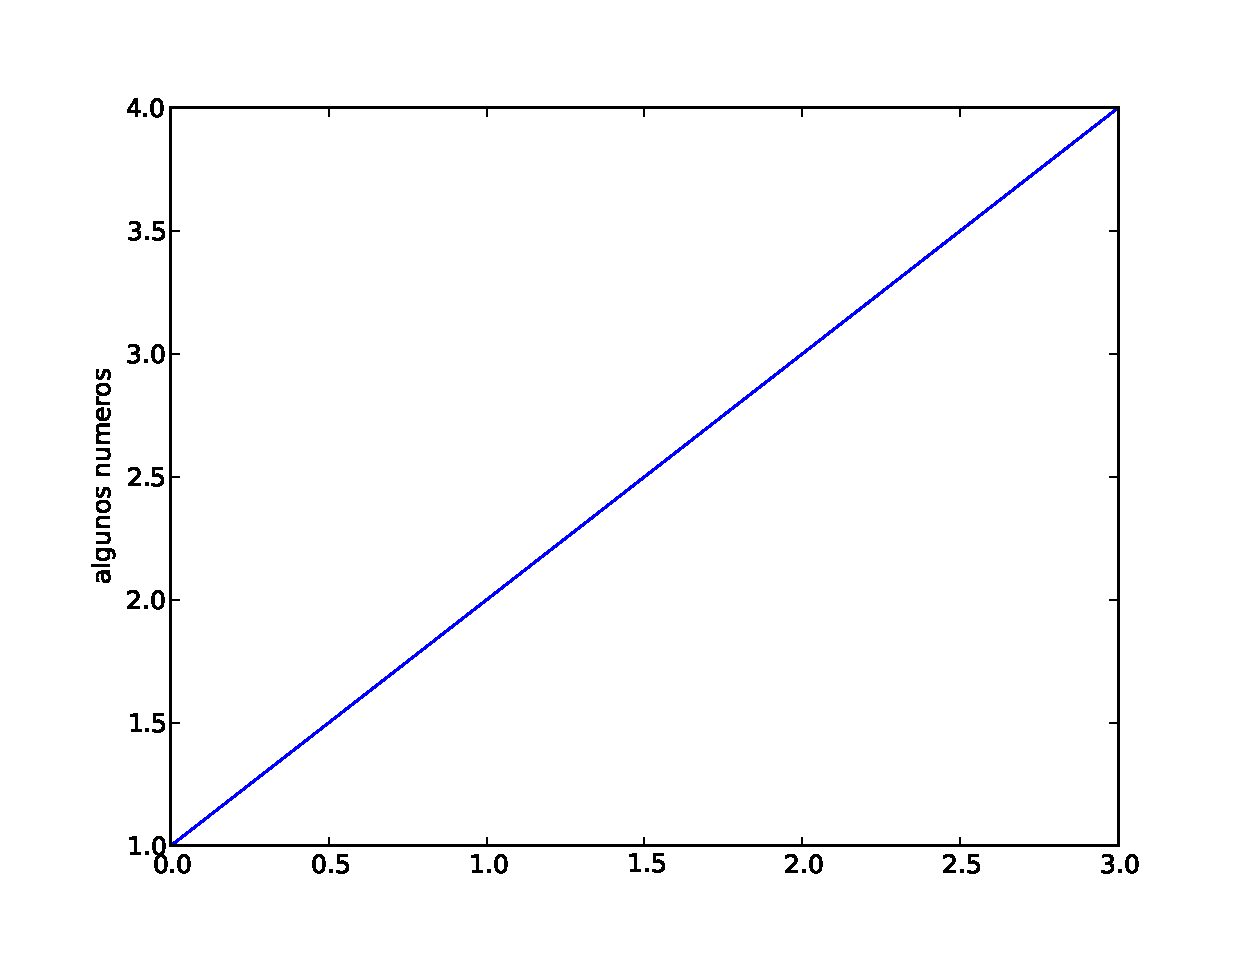
\includegraphics[scale=0.35]{plotEjercicio1.eps}
	\caption{Gráfica obtenida por el primer código.}
\end{figure}
\end{frame}
\begin{frame}[fragile]
\frametitle{Ejercicio 1}
\begin{figure}
	\centering
	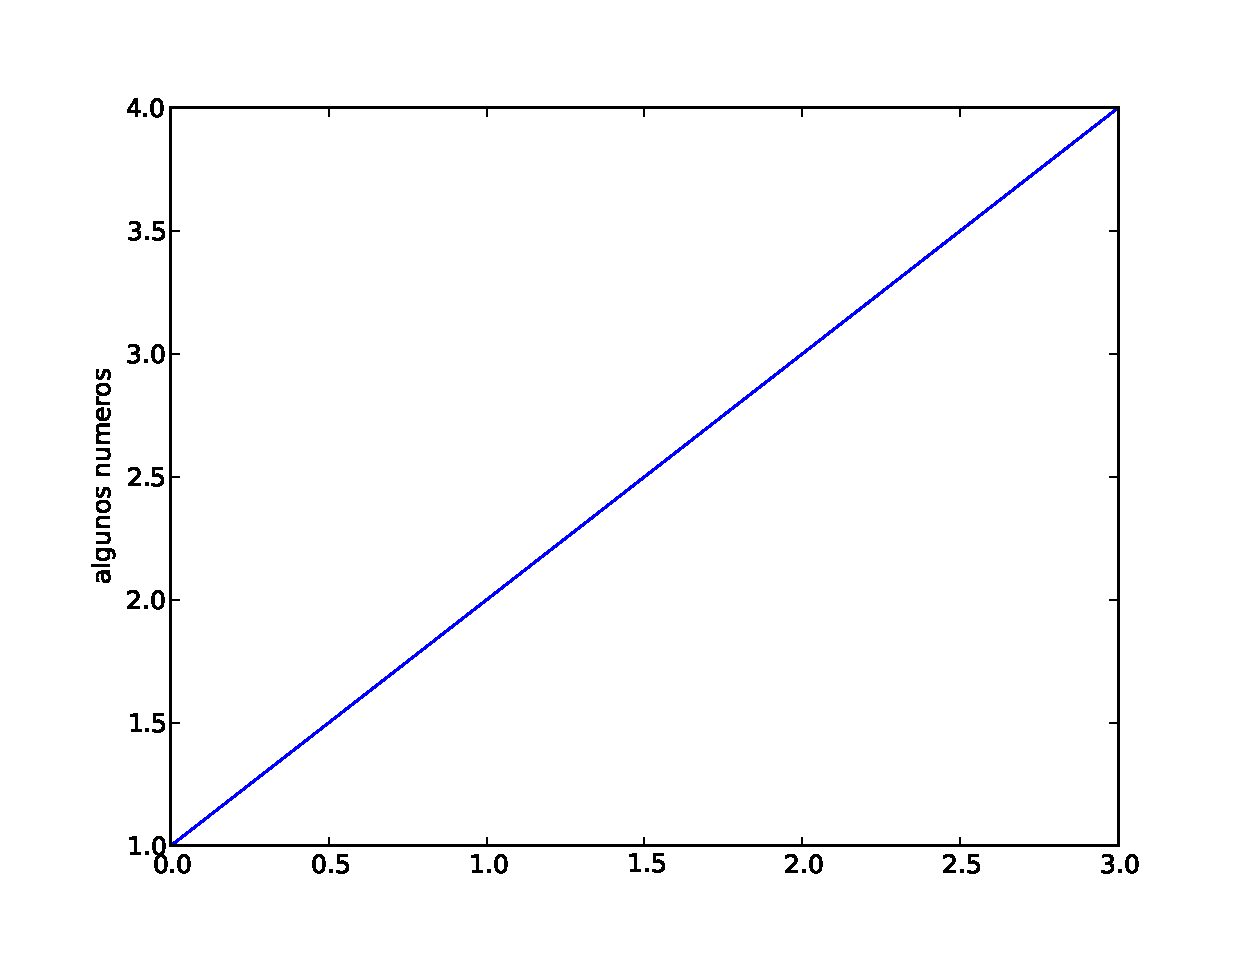
\includegraphics[scale=0.25]{plotEjercicio1.eps}
	\caption{Grafica que devuelve el primer código.}
\end{figure}
Te estarás preguntando: \textcolor{red}{ ¿por qué tenemos en el eje $x$ el rango $0-3$ y en el eje $y$ el rango  $1-4$?}
\end{frame}
\begin{frame}
\frametitle{Respuesta}
Si proporcionamos una única lista o matriz en el comando \funcionazul{plot}, entonces \funcionazul{matplotlib} asume que es una secuencia de valores de $y$, por lo que genera automáticamente los valores de $x$ para nosotros. 
\end{frame}
\begin{frame}
\frametitle{Respuesta}	
Como los índices en \python\ comienzan en $0$, el vector $x$ por defecto tiene la misma longitud que $y$, pero inicia en $0$. 
\\
\bigskip
De ahí que los datos $x$ son $[0,1,2,3]$.
\end{frame}
\begin{frame}[fragile]
\frametitle{Ejercicio 2}
\begin{lstlisting}[caption=Código con más elementos, basicstyle=\linespread{1.2}\ttfamily\small, columns=fullflexible]
import matplotlib.pyplot as plt

plt.plot([1, 2, 3, 4], [1, 4, 9, 16], 'ro')
plt.axis([0, 6, 0, 20])
plt.show()
\end{lstlisting}
\end{frame}
\begin{frame}[fragile]
\frametitle{Elementos incorporados}
\texttt{
plt.plot(\tikzmark{a1}[1,2,3,4],\tikzmark{a2}[1,4,9,16],\tikzmark{a3}'ro')
\\
\bigskip
\vspace{1.5cm}
plt.plot(\tikzmark{b1}x,\tikzmark{b2}y, \tikzmark{b3}'tipolinea-marca')
}
\begin{tikzpicture}[remember picture,overlay]
    \path[draw=blue,thick,->] ([xshift=2mm, yshift=3mm]b1) -- ([xshift=1cm, yshift=-2mm]a1);
    \path[draw=blue,thick,->] ([xshift=2mm, yshift=3mm]b2) -- ([xshift=1cm, yshift=-2mm]a2);
    \path[draw=blue,thick,->] ([xshift=2cm, yshift=3mm]b3) -- ([xshift=3mm, yshift=-2mm]a3);

\end{tikzpicture}
\end{frame}
\begin{frame}[fragile]
\frametitle{Elementos incorporados}
\texttt{
plt.axis(\tikzmark{a1}[0, 6, \tikzmark{a2}0, 20])
\\
\bigskip
\vspace{1.5cm}
plt.axis(\tikzmark{b1}x1, x2, \tikzmark{b2}y1, y2)
}
\begin{tikzpicture}[remember picture,overlay]
    \path[draw=blue,thick,->] ([xshift=2mm, yshift=3mm]b1) -- ([xshift=5mm, yshift=-2mm]a1);
    \path[draw=blue,thick,->] ([xshift=2mm, yshift=3mm]b2) -- ([xshift=2mm, yshift=-2mm]a2);
\end{tikzpicture}
\end{frame}
\begin{frame}
\frametitle{Ejercicio 2}
\begin{figure}
	\centering
	\includegraphics[scale=0.35]{plotEjercicio2.eps}
	\caption{Gráfica obtenida con dos listas de números. Nótese que los puntos no están unidos entre sí.}
\end{figure}
\end{frame}
\begin{frame}[fragile]
\frametitle{Cadena de formato}
Por cada par de argumentos $x$, $y$, existe un tercer argumento opcional, que es la cadena de formato que indica el color y tipo de línea.
\end{frame}
\begin{frame}[fragile]
\frametitle{Cadena de formato}
Las letras y los símbolos de la cadena de formato son como en MATLAB: se concatena una cadena de color con una cadena estilo de línea.
\\
\bigskip
La cadena de formato por defecto es \verb|'b-'|, que es una línea de color azul.
\end{frame}
\begin{frame}[fragile]
\frametitle{Tipos de líneas}
\fontsize{10}{10}\selectfont
\begin{tabular}{l | l}
carácter & descripción \\ \hline
\verb|'-'|	& línea sólida \\ \hline
\verb|'--'| & línea cortada \\ \hline
\verb|'-.'| & línea-punto \\ \hline
\verb|':'|	& línea de puntos \\ \hline
\verb|'.'|	& marca de punto \\ \hline
\verb|','|	& marca de pixel \\ \hline
\verb|'o'|	& marca de círculo \\ \hline
\verb|'v'|	& marca de triángulo hacia abajo \\ \hline
\verb|'^'|	& marca de triángulo hacia arriba
\end{tabular}
\end{frame}
\begin{frame}[fragile]
\frametitle{Lista de colores}
\fontsize{10}{10}\selectfont
\begin{tabular}{l | l}
carácter & color \\ \hline
\verb|'b'| & azul \\ \hline
\verb|'g'| & verde \\ \hline
\verb|'r'| & rojo \\ \hline
\verb|'c'| & cyan \\ \hline
\verb|'m'| & magenta \\ \hline
\verb|'y'| & amarillo \\ \hline
\verb|'k'| & negro \\ \hline
\verb|'w'| & blanco
\end{tabular}
\end{frame}
\begin{frame}
\frametitle{Alcance de \texttt{matplotlib}}
La librería \funcionazul{matplotlib} se limita a trabajar con listas, por lo que sería bastante acotado para el procesamiento y análisis numérico.
\\
\medskip
Por lo general, se utilizan los arreglos del módulo \funcionazul{numpy}.
\end{frame}
\begin{frame}
\frametitle{Extendiendo \texttt{matplotlib}}
De hecho, todas las secuencias se convierten en matrices de \funcionazul{numpy} internamente.
\\
\medskip
El siguiente ejemplo ilustra un trazado de líneas con varios estilos diferentes en una sola instucción utilizando arreglos.
\end{frame}
\begin{frame}[fragile]
\frametitle{Ejercicio 3}
\begin{lstlisting}[caption=Gráfica con \texttt{numpy},basicstyle=\linespread{1.2}\ttfamily\small, columns=fullflexible]
import numpy as np
import matplotlib.pyplot as plt

t = np.arange(0., 5., 0.2)
plt.plot(t, t, 'r--', t, t**2, 'bs', t, t**3, 'g^')
plt.show()
\end{lstlisting}
\end{frame}
\begin{frame}[fragile]
\frametitle{Elementos en el código}
\texttt{
t = np.arange\tikzmark{a1}(0., \tikzmark{b1}5., \tikzmark{c1}0.2)
\\
\bigskip
\vspace{1.5cm}
t = np.arange(\tikzmark{a2}inicio, \tikzmark{b2}fin, \tikzmark{c2}paso)
}
\begin{tikzpicture}[remember picture,overlay]
    \path[draw=magenta,thick,->] ([xshift=2mm, yshift=3mm]a2) -- ([xshift=5mm, yshift=-2mm]a1);
    \path[draw=magenta,thick,->] ([xshift=2mm, yshift=3mm]b2) -- ([xshift=2mm, yshift=-2mm]b1);
    \path[draw=magenta,thick,->] ([xshift=2mm, yshift=3mm]c2) -- ([xshift=5mm, yshift=-2mm]c1);
\end{tikzpicture}
\end{frame}

\begin{frame}[fragile]
\begin{figure}
	\centering
	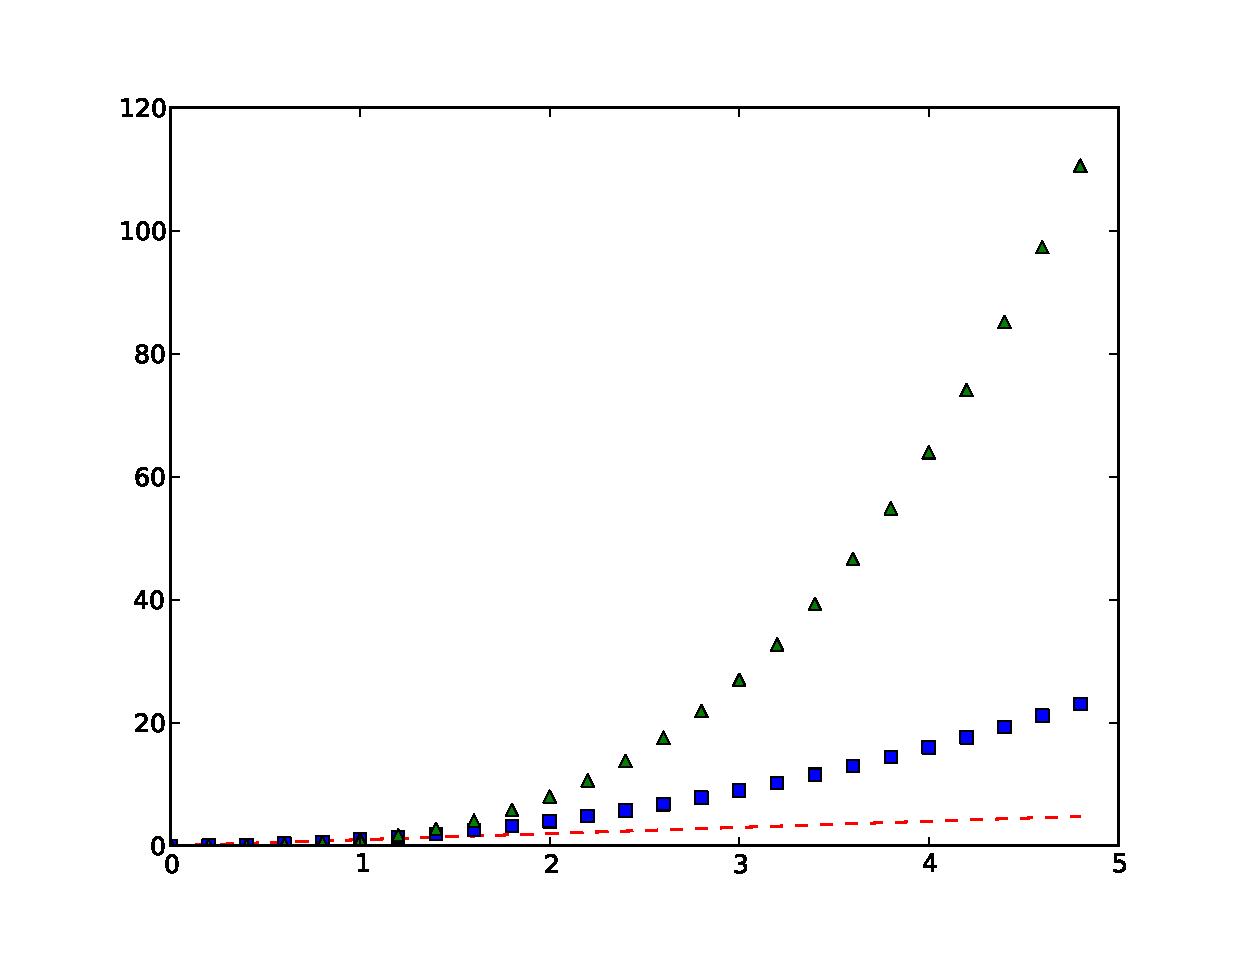
\includegraphics[scale=0.5]{plotEjercicio3.eps}
	\caption{Gráfica con tres curvas.}
\end{figure}
\end{frame}
\subsection{Trabajando con subplots}
\begin{frame}[allowframebreaks, fragile]
\frametitle{Ejercicio 4}
\begin{lstlisting}[caption=Trabajando con múltiples gráficas,basicstyle=\linespread{1.2}\ttfamily\small, columns=fullflexible]
import numpy as np
import matplotlib.pyplot as plt

def f(t):
    return np.exp(-t) * np.cos(2*np.pi*t)

t1 = np.arange(0.0, 5.0, 0.1)
t2 = np.arange(0.0, 5.0, 0.02)

plt.figure(1)
plt.subplot(211)
plt.plot(t1, f(t1), 'bo', t2, f(t2), 'k')

plt.subplot(212)
plt.plot(t2, np.cos(2*np.pi*t2), 'r--')
\end{lstlisting}
\end{frame}
\begin{frame}[fragile]
\begin{figure}
	\centering
	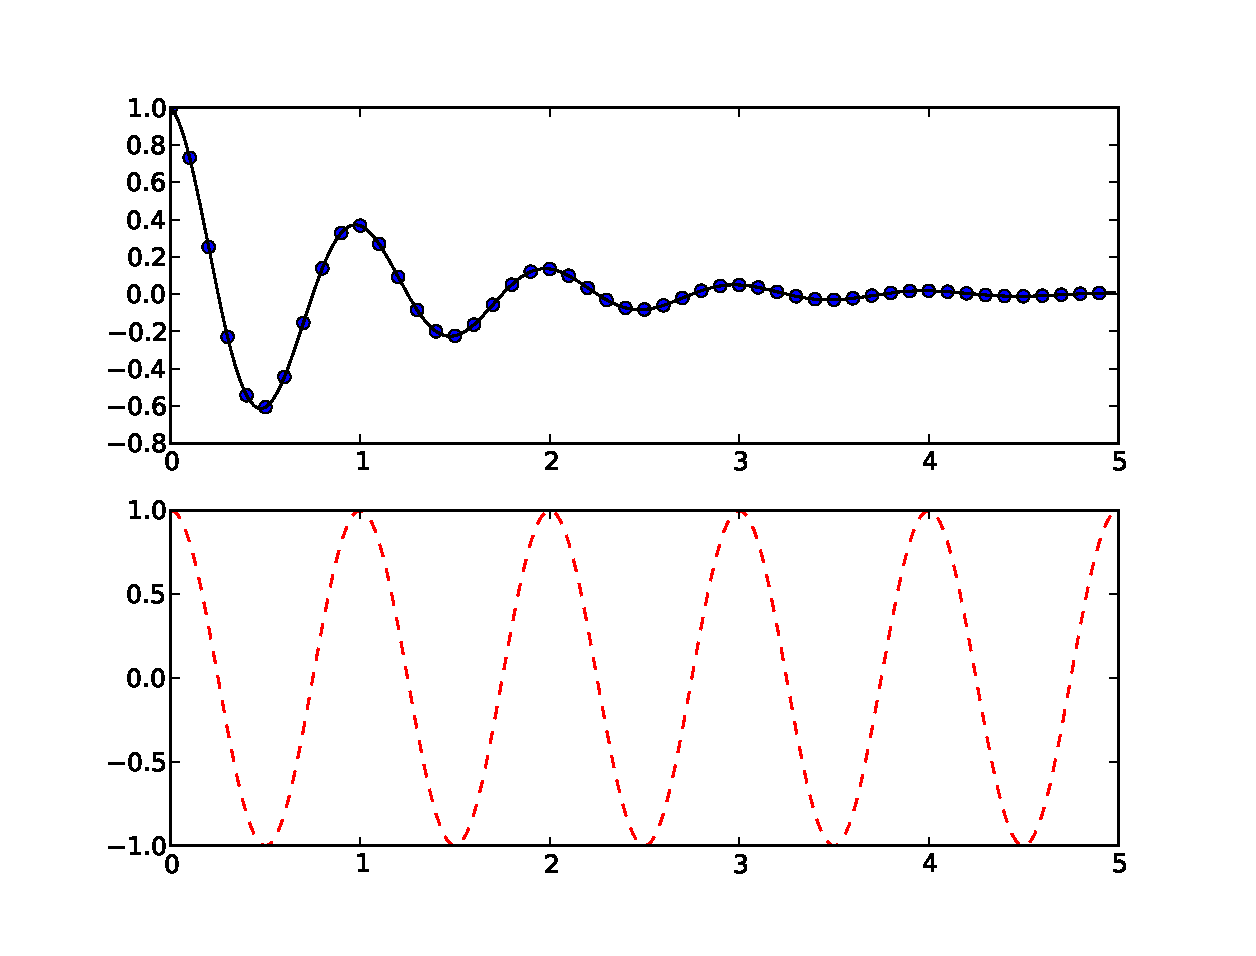
\includegraphics[scale=0.5]{plotEjercicio4.eps}
\end{figure}
\end{frame}
\begin{frame}
El comando \funcionazul{figure(\ )} aquí es opcional, ya \funcionazul{figure(1)} se crea de forma predeterminada, así mismo \funcionazul{subplot(111)} se crea de forma predeterminada si no se especifica manualmente un eje.
\end{frame}
\begin{frame}
El comando \funcionazul{subplot()} especifica \texttt{numrows, numcols, fignum} donde \texttt{fignum} varía en rango de $1$ a \texttt{numrows * numcols}.
\\
\bigskip
Las comas en el comando \funcionazul{subplot()} son opcionales si \texttt{numrows * numcols} $<10$. Por tanto \funcionazul{subplot(211)} es idéntica a la \texttt{subplot(2,1,1)}.
\end{frame}
\begin{frame}[allowframebreaks, fragile]
\frametitle{Ejercicio 5}
\begin{lstlisting}[caption=Ejemplo con subplots, basicstyle=\linespread{1.2}\ttfamily\small, columns=fullflexible]
import matplotlib.pyplot as plt

plt.figure(1)                

plt.subplot(211)        
plt.plot([1,2,3])

plt.subplot(212)         
plt.plot([4,5,6])


plt.figure(2)                
plt.plot([4,5,6])           

plt.figure(1)                
plt.subplot(211)         

plt.title('Tan facil como 1,2,3')
plt.show()
\end{lstlisting}
\end{frame}
\begin{frame}[fragile]
\begin{figure}
	\centering
	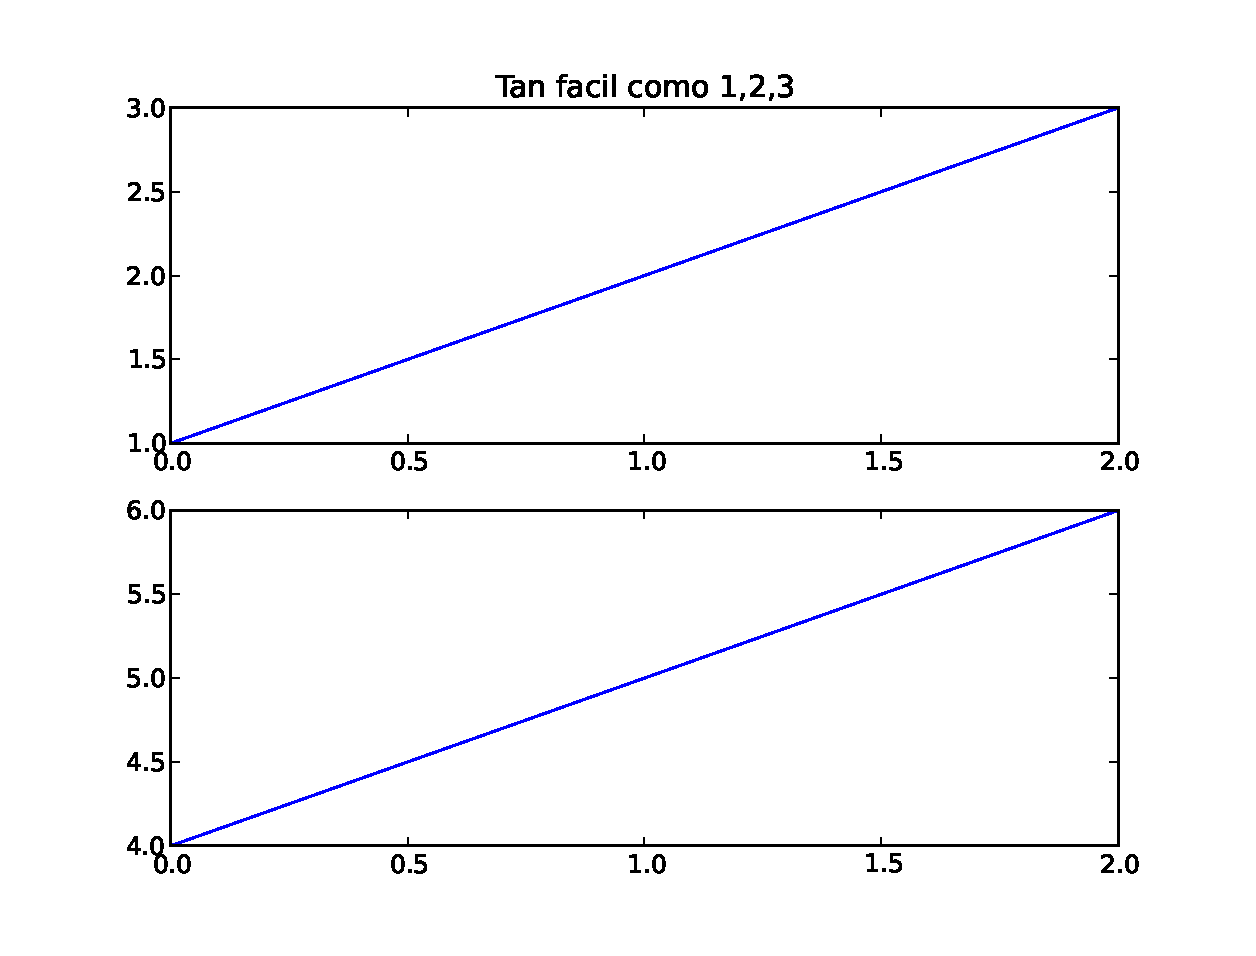
\includegraphics[scale=0.5]{plotEjercicio5_1.eps}<1>
	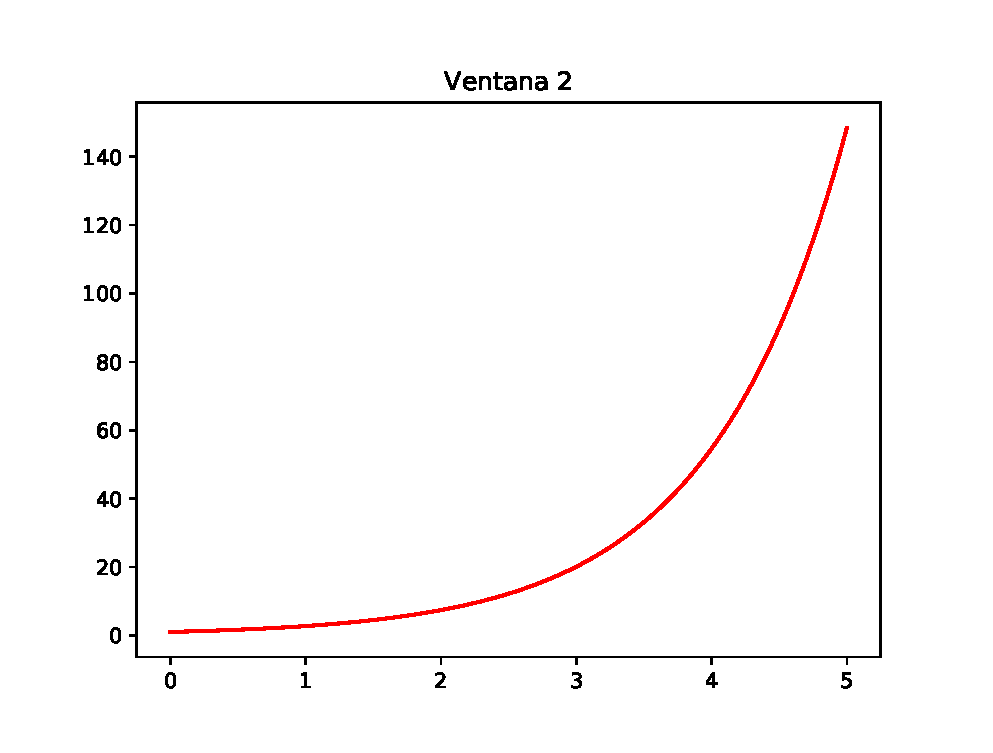
\includegraphics[scale=0.5]{plotEjercicio5_2.eps}<2>
\end{figure}
\end{frame}
\subsection{Recursos para \texttt{matplotlib}}
\begin{frame}
\frametitle{Más recursos para graficar con \python}
Lo que hemos visto es una revisión muy básica y general de cómo generar una gráfica con \python.
\end{frame}
\begin{frame}
\frametitle{Más recursos para graficar con \python}
Hay una enorme cantidad de información sobre \funcionazul{matplotlib}, que encontrarás en la página oficial de la librería, así como bastante documentación, ejemplos y elementos para extender completamente esta herramienta.
\end{frame}
\begin{frame}
Se les proporcionará una guía breve de graficación, con la intención de que revisen casos prácticos aplicados a la física. Para cada gráfica que usemos más adelante en el curso, tendrán oportunidad de agregar más elementos que ustedes consideren.
\end{frame}
\begin{frame}
\frametitle{Ejemplos de tipos de gráficas}
\begin{figure}
	\centering
	\only<1>{
	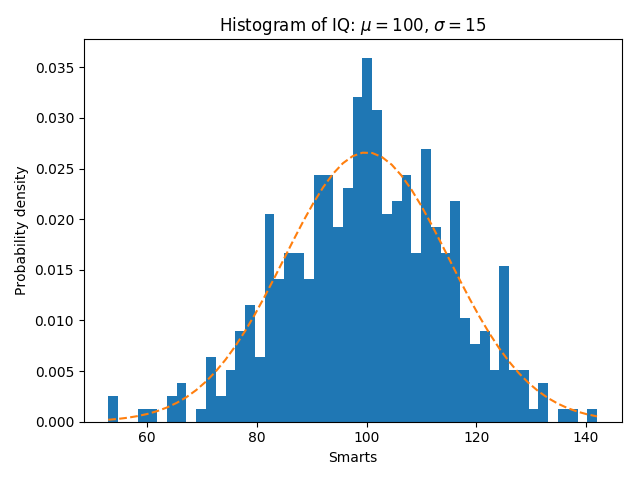
\includegraphics[scale=0.5]{Imagenes/sphx_glr_histogram_features_001.png}
	\caption{Histograma}
	}
	\only<2>{
	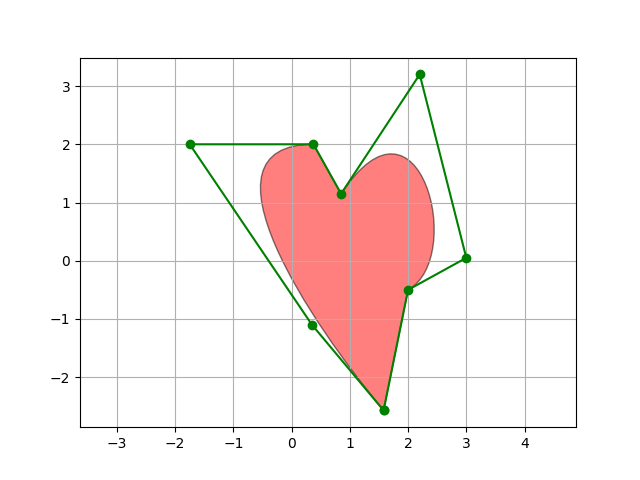
\includegraphics[scale=0.5]{Imagenes/sphx_glr_path_patch_001.png}
	\caption{Contorno}
	}
	\only<3>{
	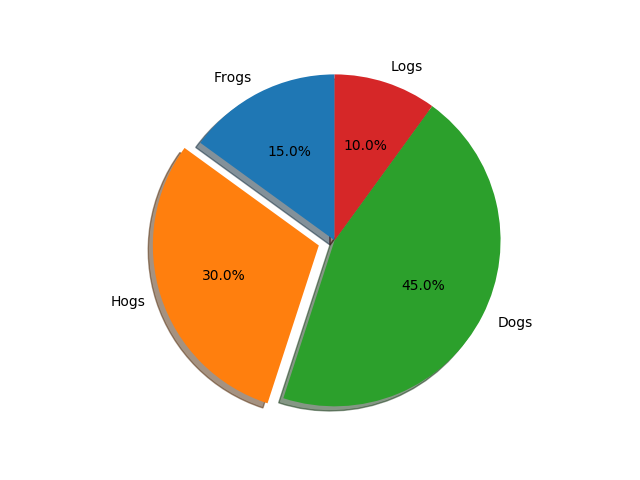
\includegraphics[scale=0.5]{Imagenes/sphx_glr_pie_features_001.png}
	\caption{Pastel}
	}
	\only<4>{
	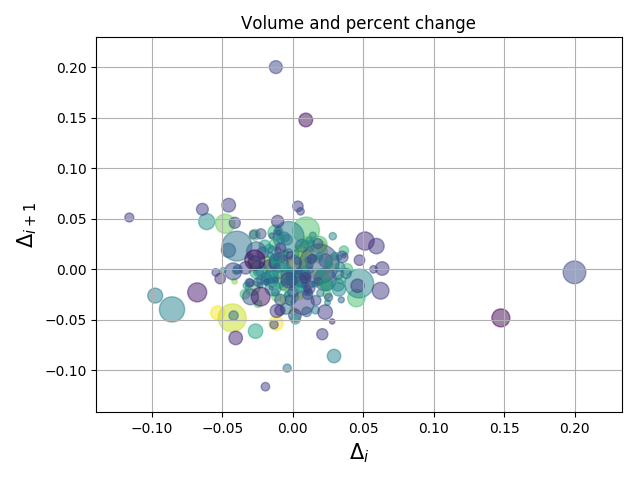
\includegraphics[scale=0.5]{Imagenes/sphx_glr_scatter_demo2_001.png}
	\caption{Dispersión}
	}
	\only<5>{
	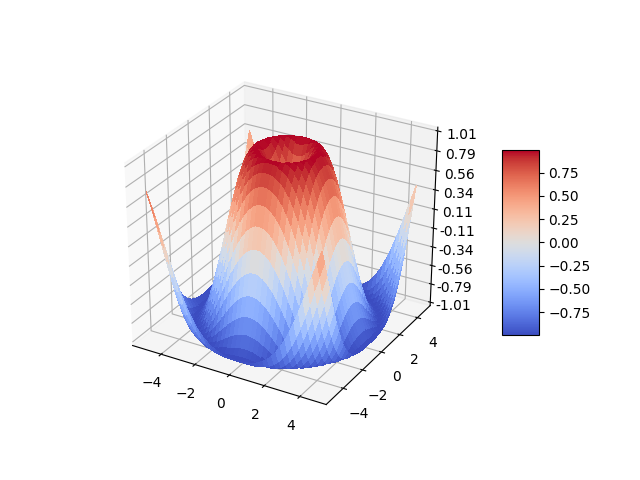
\includegraphics[scale=0.5]{Imagenes/sphx_glr_surface3d_001.png}
	\caption{Superficie 3D}
	}
	\only<6>{
	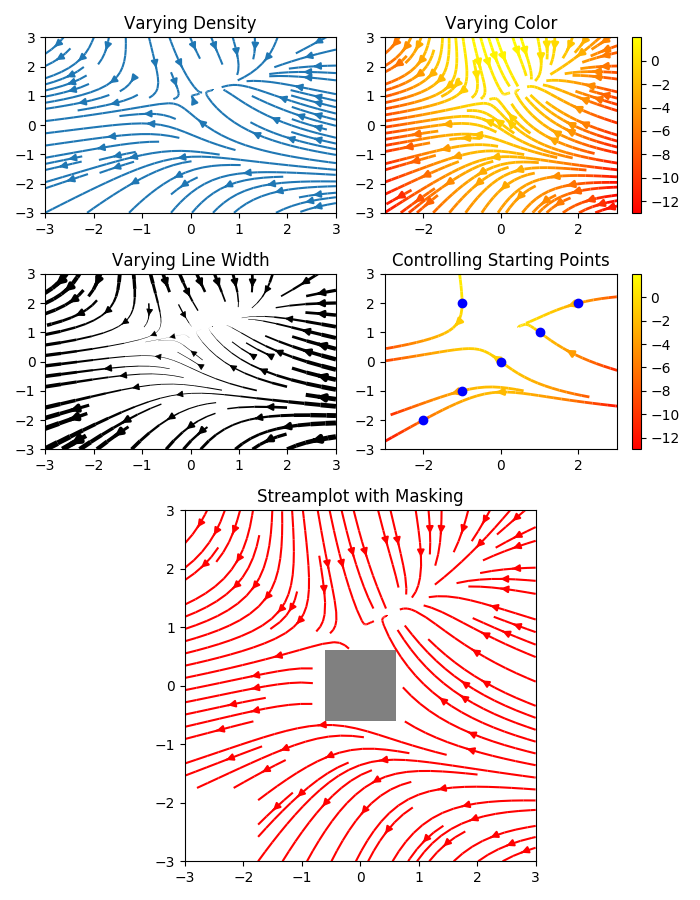
\includegraphics[scale=0.4]{Imagenes/sphx_glr_plot_streamplot_001.png}
	\caption{Campos vectoriales}
	}
\end{figure}
\end{frame}
\section{Ejercicios de Mecánica}
\frame{\tableofcontents[currentsection, hideothersubsections]}
\subsection{El oscilador armónico}
\begin{frame}
\frametitle{Un primer problema de Mecánica}
Supongamos que tenemos una partícula de masa $m$ que está confinada a moverse a lo largo del eje $x$, bajo una fuerza $f(x)$. Sabemos de la ley de Newton que
\begin{equation}\label{Eqfuerza}
f = ma = m \dfrac{dv}{dt}
\end{equation}
donde $a$ es la aceleración y $v$ la velocidad de la partícula respectivamente, $t$ es el tiempo.
\end{frame}
\begin{frame}
\frametitle{Un primer problema de Mecánica}
Si dividimos el tiempo en pequeños intervalos iguales $\tau = t_{i + 1} - t_{i}$, sabemos que la velocidad en el tiempo $t_{i}$, está dada de manera aproximada por el promedio de la velocidad en el intervalo de tiempo $[t_{i}, t_{i + 1}]$
\end{frame}
\begin{frame}
\frametitle{Un primer problema de Mecánica}
Por lo que
\begin{equation}\label{Eqvelocidad}
v_{i} \simeq \dfrac{x_{i+1}-x_{i}}{t_{i+1}-t_{i}} = \dfrac{x_{i+1}-x_{i}}{\tau}
\end{equation}
\end{frame}
\begin{frame}
\frametitle{Un primer problema de Mecánica}
La aceleración de la partícula es aproximadamente el promedio de la aceleración en el mismo intervalo
\begin{equation}\label{Eqaceleracion}
a_{i} \simeq \dfrac{v_{i+1}-v_{i}}{t_{i+1}-t_{i}} = \dfrac{v_{i+1}-v_{i}}{\tau}
\end{equation}
donde $\tau$ es muy pequeño.
\end{frame}
\begin{frame}
\frametitle{Hallar la posición y velocidad}
El algoritmo más sencillo para determinar la posición y velocidad de la partícula en el tiempo $t_{1i+1}$, a partir de las cantidades correspondientes al tiempo $t_{i}$, se obtiene luego de combinar las ecuaciones (\ref{Eqfuerza}), (\ref{Eqvelocidad}) y (\ref{Eqaceleracion}), por lo que
\begin{eqnarray}
x_{i+1} &=& x_{i} + \tau v_{i} \label{Eqposicion} \\
v_{i+1} &=& v_{i} + \dfrac{\tau}{m} f_{i} \label{Eqvelocidadr}
\end{eqnarray}
donde $f_{i} = f(x_{i})$
\end{frame}
\begin{frame}
\frametitle{Hallar la posición y velocidad}
Si se proporcionan la posición inicial y la velocidad inicial de la partícula, para luego calcular las cantidades correspondientes en algún momento posterior (problema de valor inicial), podemos obtenerlas de forma recursiva a partir del algoritmo dado en las ecuaciones (\ref{Eqposicion}) y (\ref{Eqvelocidadr}).
\end{frame}
\begin{frame}
\frametitle{Ejercicio 1: Oscilador mecánico}
Por simplicidad, consideremos que la fuerza es $f(x) = -kx$, donde $k$ es la constante del resorte. Usemos $m=k=1$.
\\
\bigskip
\pause
Queremos describir la posición y velocidad de la partícula en un intervalo de tiempo de 100 segundos.
\\
\bigskip
\pause
Las condiciones iniciales son las siguientes: $x(t=0) = 0$ y $v(t=0) = 1$.
\end{frame}
\begin{frame}[<+->]
\frametitle{Resolviendo el problema con Python}
¿Qué es lo que tenemos?
\begin{itemize}
\item El intervalo de tiempo de $[0,100]$ segundos.
\item La posición inicial y velocidad inicial.
\item Las expresiones para calcular los $x_{i+1}$ y $v_{i+1}$
\end{itemize}
\visible<4->{¿Qué nos falta?}
\end{frame}
\begin{frame}[fragile]
\frametitle{Lo que nos falta}
\begin{itemize}[<+->]
\item Calcular la posición y velocidad para cada segundo en el intervalo $[0,100]$.
\item Guardar esos valores en un algún lado.
\item Graficar los resultados.
\end{itemize}
\end{frame}
\begin{frame}[fragile]
\frametitle{Uso de los módulos para nuestro programa}
Para graficar con el módulo \funcionazul{matplotlib} incluido en \python, necesitamos llamar a la librería \funcionazul{pyplot}, para acortar la escritura, usamos un \emph{alias}, en este caso \texttt{plt}.
\begin{lstlisting}[caption=Importando librerías, basicstyle=\linespread{1.2}\ttfamily\small, columns=fullflexible]
import matplotlib.pyplot as plt
from math import pi
\end{lstlisting}
\end{frame}
\begin{frame}[fragile]
\frametitle{Usando lo que conocemos}
\begin{lstlisting}[caption=Información que nos da el enunciado, basicstyle=\linespread{1.2}\ttfamily\small, columns=fullflexible]
n = 100

x = []
v = []

dt = 2* pi/n

x.append(0)
v.append(1)
\end{lstlisting}
\end{frame}
\begin{frame}[fragile]
\frametitle{Ciclo de iteración para los nuevos valores}
Como la fuerza en este caso es del tipo $f(x) = -k \; x$, tenemos un cambio de signo en el segundo sumando de $vi$.
\pause
\begin{lstlisting}[caption=Calculando nuevos valores, basicstyle=\linespread{1.2}\ttfamily\small, columns=fullflexible]
for i in range(n-1):
    xi = x[i] + v[i]*dt
    vi = v[i] - x[i]*dt
    
    x.append(xi)
    v.append(vi)
\end{lstlisting}
\end{frame}
\begin{frame}
\frametitle{Almacenando los valores nuevos}
Conforme se itera en el ciclo \funcionazul{for ... in}, se obtienen nuevos valores tanto de la posición como de la velocidad, y se almacenan en las respectivas listas.
\\
\bigskip
Desplegar el contenido de las dos columnas en la termina, no nos brinda una forma de apreciar el resultado, entonces lo que haremos, es graficar esos datos.
\end{frame}
\begin{frame}[fragile]
\frametitle{Crear la gráfica}
\begin{lstlisting}[caption=Graficando los resultados, basicstyle=\linespread{1.2}\ttfamily\small, columns=fullflexible]
plt.plot(x, "ro-", label="Posicion")
plt.plot(v, "b+-", label="Velocidad")
plt.legend(loc="upper right")
plt.xlabel("tiempo")
plt.show()
\end{lstlisting}
\end{frame}
\begin{frame}
\frametitle{Resultado del problema}
\begin{figure}
	\centering
	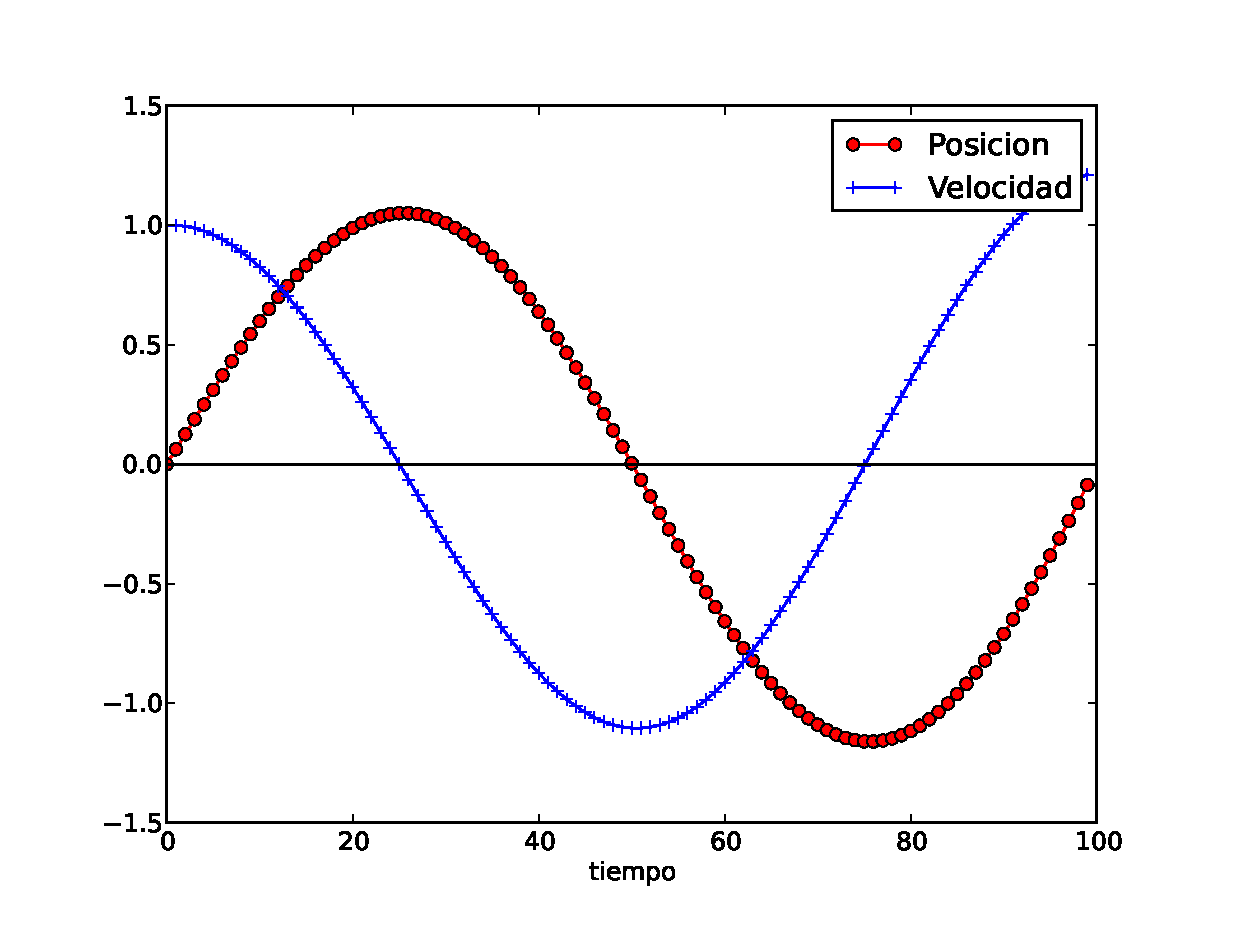
\includegraphics[scale=0.5]{Imagenes/EjerMecanica01.eps} 
\end{figure}
\end{frame}
\subsection{Efecto de la resistencia del aire}
\begin{frame}
\frametitle{Ejecicio 2: Efecto de la resistencia del aire}
La bicicleta es una forma muy eficiente de transporte, este es un hecho bien conocido por cualquier persona que monta una. 
\\
\bigskip
Nuestro objetivo en este ejercicio es comprender los factores que determinan la velocidad máxima de una bicicleta y estimar la velocidad de un caso real.
\end{frame}
\begin{frame}
\frametitle{Ejecicio 2: Efecto de la resistencia del aire}
Comenzaremos haciendo caso omiso de la fricción; tendremos que añadirlo al final, por supuesto, pero debemos primero entender cómo lidiar con el caso más simple y sin fricción.
\end{frame}
\begin{frame}
\frametitle{Ecuación de movimiento}
La ecuación de movimiento corresponde a la segunda ley de Newton, que escribimos de la forma
\begin{equation}\label{EqNewton2}
\dfrac{dv}{dt} = \dfrac{F}{m}
\end{equation}
\end{frame}
\begin{frame}
\frametitle{Ecuación de movimiento}
\begin{equation*}
\dfrac{dv}{dt} = \dfrac{F}{m}
\end{equation*}
donde
\setbeamercolor{item projected}{bg=green!70!black,fg=white}
\setbeamertemplate{enumerate items}[circle]
\begin{enumerate}[<+->]
\item $v$ es la velocidad.
\item $m$ es la masa de la combinación de la bicicleta-conductor.
\item $t$ es el tiempo.
\item $F$ es la fuerza en la bicicleta que viene del esfuerzo del conductor (supondremos que la bicicleta se mueve sobre un terreno plano)
\end{enumerate}
\end{frame}
\begin{frame}
\frametitle{Definir la fuerza}
Tratar correctamente a $F$ se complica por la mecánica de la bicicleta, ya que la fuerza ejercida por el ciclista se transmite a las ruedas por medio del plato, engranajes, cadena, etc.
\\
\medskip
Esto hace que sea muy difícil derivar una expresión exacta para $F$.
\end{frame}
\begin{frame}
\frametitle{Definir la fuerza}
Sin embargo, hay otra manera de abordar este problema que evita la necesidad de conocer la fuerza.
\\
\medskip
Este enfoque alternativo implica la formulación del problema en términos de la potencia generada por el ciclista.
\end{frame}
\begin{frame}
\frametitle{Comparando la potencia}
Estudios fisiológicos en ciclistas de carreras han demostrado que éstos atletas son capaces de producir una potencia de salida de aproximadamente $400$ watts durante largos períodos de tiempo ($\sim 1$ h)
\end{frame}
\begin{frame}
\frametitle{Usando la potencia generada}
Usando las ideas de trabajo-energía podemos reescribir (\ref{EqNewton2}) como
\begin{equation}\label{EqPotencia}
\dfrac{dE}{dt} = P
\end{equation}
donde $E$ es la energía total, $P$ es la potencia de salida del ciclista. 
\end{frame}
\begin{frame}
\frametitle{Expresando la energía}
Para un trayecto plano la energía es totalmente cinética, es decir,
\[ E = \frac{1}{2} m v^{2} \]
y además
\[ \frac{dE}{dt} = mv (\frac{dv}{dt}) \]
\pause
usando esto en (\ref{EqPotencia}), resulta
\begin{equation}\label{EqPotenciavel}
\dfrac{dv}{dt} = \dfrac{P}{mv}
\end{equation}
\end{frame}
\begin{frame}
\frametitle{Expresando la energía}
Si $P$ es una constante, la ecuación (\ref{EqPotenciavel}), se puede resolver de manera analítica, rearreglando términos:
\begin{equation}\label{EqIntegral}
\int_{v_{0}}^{v} v' dv' = \int_{0}^{t} \dfrac{P}{m} dt'
\end{equation}
donde $v_{0}$ es la velocidad de la bicicleta en $t=0$. 
\end{frame}
\begin{frame}
\frametitle{Expresando la energía}
Integrando ambos lados de la ecuación y resolviendo para $v$, tenemos
\begin{equation}\label{Eqvres}
v = \sqrt{v_{0}^{2} + 2 \: P \: \dfrac{t}{m}}
\end{equation}
\end{frame}
\begin{frame}
\frametitle{Pasando al código}
Como ya tenemos un conjunto de elementos necesarios para resolver el ejercicio, ahora nos enfocamos a traducir en el lenguaje de \python, lo necesario para la solución.
\\
\bigskip
Recuerda que debemos de almacenar los valores nuevos de velocidad, como se calcula un valor nuevo por cada unidad de tiempo, entonces ya tenemos un par de variables para graficar.
\end{frame}
\begin{frame}[allowframebreaks, fragile]
\frametitle{Considera lo siguiente}
\begin{lstlisting}[caption=Información inicial del problema, style=FormattedNumber, basicstyle=\linespread{1.2}\ttfamily=\small, columns=fullflexible]
import matplotlib.pyplot as plt
from math import sqrt

t = []
v = []

dt = 1

potencia = 400
masa = 70
tmax = 200
nmax = tmax/dt


t.append(0)
v.append(4)
\end{lstlisting}
\end{frame}
\begin{frame}[fragile]
\frametitle{Calculando nuevos valores}
\begin{lstlisting}[caption=Ciclo para los nuevos valores de velocidad, style=FormattedNumber,basicstyle=\linespread{1.1}\ttfamily=\small, columns=fullflexible]
for i in range(int(tmax/dt)):
    ti = t[i-_1_] + dt
    vi = sqrt(v[i]**2 + (2 * potencia * dt)/masa)
    
    
    t.append(ti)
    v.append(vi)
\end{lstlisting}
\end{frame}
\begin{frame}[fragile]
\frametitle{Rutina de graficación}
\begin{lstlisting}[caption=Rutina para graficar los resultados, style=FormattedNumber,basicstyle=\linespread{1.2}\ttfamily=\small, columns=fullflexible]
plt.plot(v, "r-")
plt.xlabel("tiempo [s]")
plt.ylabel("velocidad m/s")
plt.title("Velocidad del ciclista")
plt.show()
\end{lstlisting}
\end{frame}
\begin{frame}
\frametitle{Resultado de la velocidad sin fricción}
\begin{figure}
	\centering
	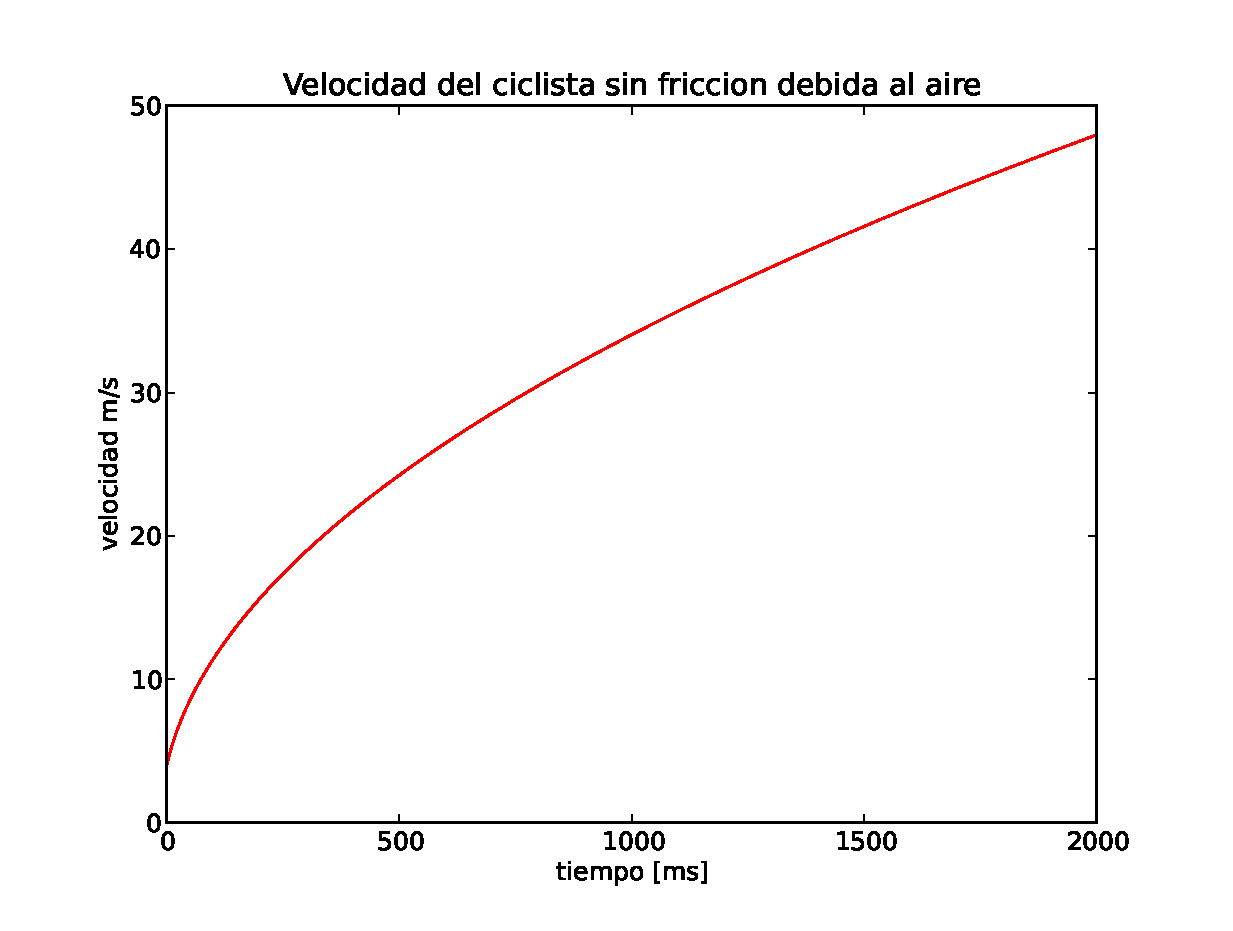
\includegraphics[scale=0.5]{EjerBicicleta01.eps}
\end{figure}
\end{frame}
\begin{frame}
\frametitle{Interpretación}
\textbf{¿Es congruente la solución numérica con la física?}
\\
\bigskip
\pause
La solución de la ecuación de movimiento (\ref{EqPotenciavel}) es correcta, pero nuestro trabajo no concluye aquí:
\pause
\begin{alertblock}{La física no checa}
La solución predice que la velocidad del ciclista se incrementará sin límite para tiempos muy largos.
\end{alertblock}
\end{frame}
\begin{frame}
\frametitle{Ajuste en el modelo inicial}
Vamos a corregir este resultado: cuando se generaliza el modelo se debe de incluir el efecto de la resistencia del aire.
\\
\bigskip
El nuevo término que vamos a añadir a la ecuación de movimiento nos obliga a desarrollar una solución numérica, así que con eso en mente se considera un tratamiento numérico de (\ref{EqPotenciavel})
\end{frame}
\begin{frame}
\frametitle{Abordaje numérico}
Comenzamos con la forma de diferencias finitas para la derivada de la velocidad
\begin{equation}\label{Eqderivada}
\dfrac{dv}{dt} \simeq \dfrac{v_{i+1}-v_{i}}{\Delta t}
\end{equation}
donde asumimos que $\Delta t$ es paso discreto pequeño, y $v_{i}$ es la velocidad al tiempo $t_{i} \equiv i \Delta t$.
\end{frame}
\begin{frame}
\frametitle{Abordaje numérico}
Por lo que de la ecuación (\ref{EqPotenciavel})
\begin{equation}\label{Eqveli+1}
v_{i+1} = v_{i} + \dfrac{P}{m v_{i}} \Delta t
\end{equation}
\end{frame}
\begin{frame}
\frametitle{Calculando la velocidad}
Dada la velocidad en un tiempo $i$ (es decir, $v_{i}$), podemos usar (\ref{Eqveli+1}) para calcular un valor \textit{aproximado} de la velocidad en el siguiente paso $v_{i+1}$.
\end{frame}
\begin{frame}
\frametitle{Calculando la velocidad}
Si conocemos la velocidad inicial $v_{0}$, podemos obtener $v_{1}$, $v_{2}$, y así sucecivamente.
\\
\bigskip
Ahora hay que introducir en la ecuación, los parámetros de fricción debida al aire.
\end{frame}
\begin{frame}
\frametitle{Considerando la fricción del aire}
La fuerza debida a la fricción puede aproximarse de manera inicial como
\begin{equation}\label{EqFfriccion}
F_{a} \simeq - B_{1} \: v - B_{2} \: v^{2}
\end{equation}
\end{frame}
\begin{frame}
\frametitle{Considerando la fricción del aire}
\begin{equation*}
F_{a} \simeq - B_{1} \: v - B_{2} \: v^{2}
\end{equation*}
Para velocidades muy bajas, el primer término es el que domina, y su coeficiente $B_{1}$ se puede calcular para objetos con formas sencillas.
\end{frame}
\begin{frame}
\frametitle{Considerando la fricción del aire}
\begin{equation*}
F_{a} \simeq - B_{1} \: v - B_{2} \: v^{2}
\end{equation*}
Para una velocidad razonable $v^{2}$ el término domina sobre los demás, pero el coeficiente $B_{2}$ no puede calcularse exactamente en objetos sencillos como una pelota de beisbol, menos para una bicicleta.
\end{frame}
\begin{frame}
\frametitle{Primera aproximación}
Podemos aproximar el valor de $B_{2}$ como sigue:
\\
\medskip
Si un objeto se mueve a través de la atmósfera, entonces debe empujar al aire delante fuera del camino.
\end{frame}
\begin{frame}
\frametitle{Primera aproximación}
La masa de aire movido en el tiempo $dt$ es
\[m_{aire} \sim \rho \: A \: v \: dt \]
donde $\rho$ es la densidad del aire y $A$ el área frontal del objeto. 
\\
\bigskip
\pause
A este aire se le da una velocidad de orden $v$, y por lo tanto, su energía cinética es
\[E_{aire} \sim m_{aire} \: v^{2} /2 \]
\end{frame}
\begin{frame}
\frametitle{Primera aproximación}
Este es también el trabajo realizado por la fuerza de arrastre (la fuerza sobre el objeto debido a la resistencia del aire) en el tiempo $dt$, por lo $F_{a} \: v \: dt = E_{aire}$.
\\
\bigskip
Poniendo todo esto junto nos encontramos con:
\[ F_{a} \simeq - C \: \rho \: A \: v^{2} \]
\end{frame}
\begin{frame}
\frametitle{Coeficiente de arrastre}
De la expresión
\[ F_{a} \simeq - C \: \rho \: A \: v^{2} \]
Tenemos que $C$ es el coeficiente de arrastre, podemos argumentar que tiene un valor de $0.5$ (¿cómo lo demostrarías?).
\end{frame}
\begin{frame}
\frametitle{Coeficiente de arrastre}
Recordemos que estamos haciendo una primera aproximación, si nos interesa contar con una expresión que determine la correcta relación de $F_{a}$ con $v$ y $A$, entonces tendremos que hacer mediciones en un túnel de viento, para utilizar el valor correcto de $C$.
\end{frame}
\begin{frame}
\frametitle{Nueva expresión para la velocidad}
Incluyendo este término en la expresión para la velocidad
\begin{equation}\label{Eqvelifriccion}
v_{i+1} = v_{i} + \dfrac{P}{m v_{i}} \Delta t - \dfrac{C \rho A v_{i}^{2}}{m} \Delta t
\end{equation}
Considera los siguientes valores:
\setbeamercolor{item projected}{bg=green!70!black,fg=white}
\setbeamertemplate{enumerate items}[circle]
\begin{enumerate}[<+->]
\item Coeficiente de arrastre: $C = 0.5$
\item Sección de área frontal: $0.33 \: \si{\square\meter}$
\item Masa del sistema ciclista-bicicleta: $70 \: \si{\kilogram}$
\item Velocidad inicial: $4 \: \si{\meter\per\second}$
\item Incremento en el tiempo: $\Delta \: t = 0.1 \: \si{\second}$
\end{enumerate}
\end{frame}
\begin{frame}[fragile]
\frametitle{Agregando código}
Agrega lo siguiente en tu código, te recomendamos guardar con otro nombre tu archivo.
\begin{lstlisting}[caption=Valores para el caso con fricción, style=FormattedNumber, basicstyle=\linespread{1.1}\ttfamily=\small, columns=fullflexible]
v_2_ = []

masa = 70

A = 0.33

C = 0.5
\end{lstlisting}
\end{frame}
\begin{frame}[fragile]
\frametitle{Agregando código}
\begin{lstlisting}[caption=En el ciclo \texttt{for ... in}, style=FormattedNumber, basicstyle=\linespread{1.1}\ttfamily=\small, columns=fullflexible]
vc = v_2_[i-_1_] + potencia * dt / (masa * v_2_[i-_1_]) - (C * A * v_2_[i-_1_] ** 2) * dt/masa
    
v_2_.append(vc)
\end{lstlisting}
\end{frame}
\begin{frame}[fragile]
\frametitle{Agregando código}
\begin{lstlisting}[caption=Para la gráfica, style=FormattedNumber, basicstyle=\linespread{1.1}\ttfamily=\small, columns=fullflexible]
plt.plot(v, "r-", label="Velocidad sin friccion")
plt.plot(v_2_, "b-", label="Velocidad con friccion")
plt.legend(loc="upper left")
\end{lstlisting}
\end{frame}
\begin{frame}
\frametitle{Comparando velocidades}
\begin{figure}
	\centering
	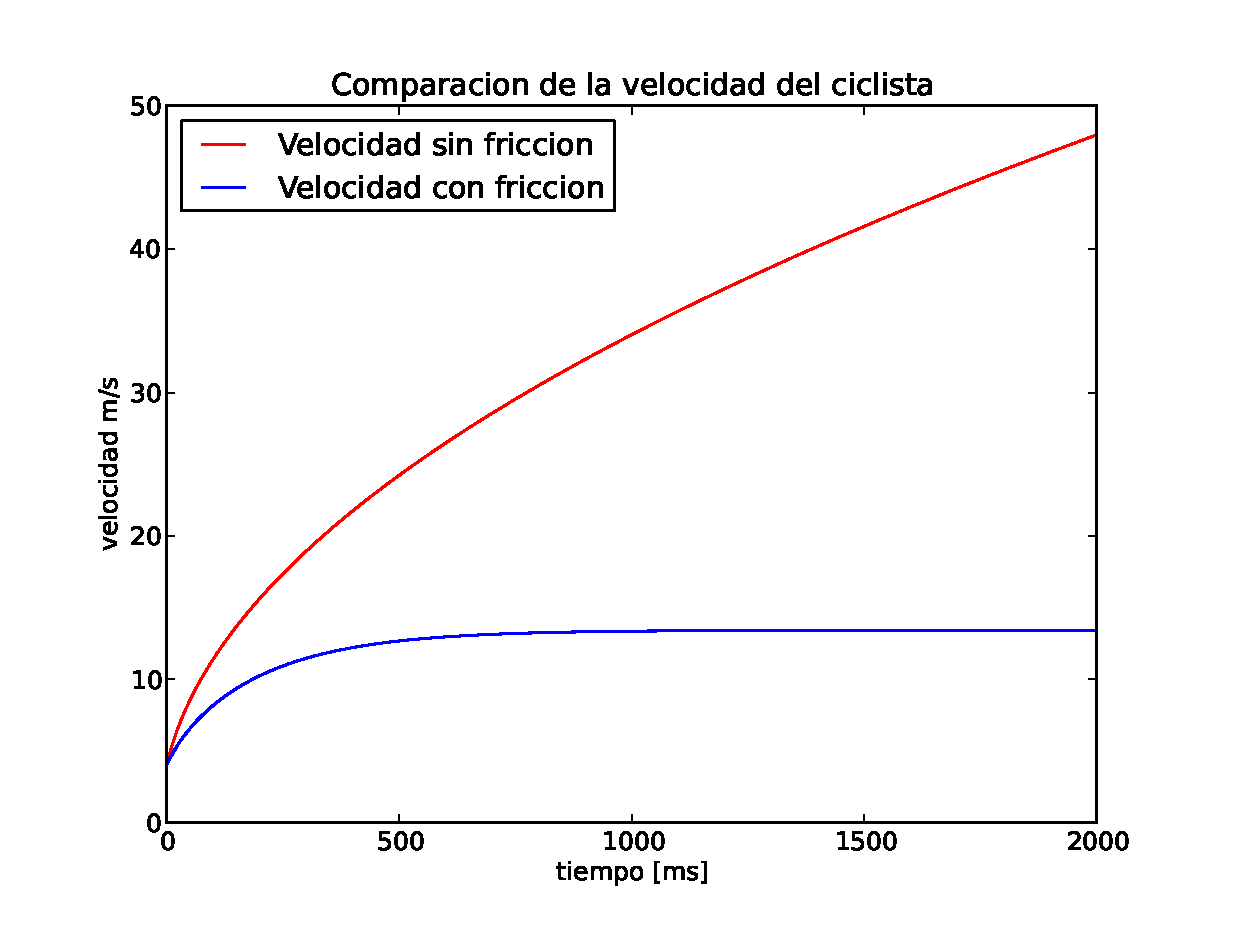
\includegraphics[scale=0.5]{EjerBicicleta02.eps}
\end{figure}
\end{frame}
\begin{frame}
\frametitle{Conclusión}
Con este ejercicio encontramos que no necesariamente una solución que funcione desde el punto de vista informático, tendrá consistencia con la física.
\\
\bigskip
Será nuestra tarea verificar que esa congruencia se mantenga en nuestros algoritmos y soluciones.
\end{frame}
\end{document}